\documentclass{article}
\usepackage[utf8]{inputenc}
\usepackage{amsmath, amssymb, physics, graphicx}
\usepackage{tikz}
\usepackage{caption}
\usetikzlibrary{arrows.meta, decorations.pathmorphing}

\title{Desarrollo de la Ecuación de Vorticidad en Ductos}
\author{Tu Nombre}
\date{\today}

\begin{document}

\maketitle

\section{Introducción}

La vorticidad es una magnitud clave en el estudio de la dinámica de fluidos, especialmente en flujos con geometría compleja. En esta nota se analiza el desarrollo y la evolución de la vorticidad en dos situaciones comunes: un ducto curvado (generación de vorticidad secundaria) y un ducto que se ensancha (difusión de vorticidad axial).

\vspace{1em}
Partimos de la ecuación de Navier-Stokes para flujo incompresible y derivamos la ecuación de vorticidad aplicando el operador rotacional.

\section{Ecuaciones Base}

\subsection{Navier-Stokes para Flujo Incompresible}
\begin{equation}
    \frac{D\vec{u}}{Dt} = -\frac{1}{\rho}\nabla p + \nu \nabla^2 \vec{u}, \quad \text{con} \quad \nabla \cdot \vec{u} = 0
\end{equation}

\subsection{Ecuación de Vorticidad}
Aplicando el rotacional:
\begin{equation}
    \frac{D\vec{\omega}}{Dt} = (\vec{\omega} \cdot \nabla)\vec{u} - (\vec{u} \cdot \nabla)\vec{\omega} + \nu \nabla^2 \vec{\omega}
\end{equation}

Para flujo incompresible, se simplifica a:
\begin{equation}
    \frac{D\vec{\omega}}{Dt} = (\vec{\omega} \cdot \nabla)\vec{u} + \nu \nabla^2 \vec{\omega}
\end{equation}


donde:

\begin{itemize}
    \item $(\vec{\omega} \cdot \nabla)\vec{u}$: Estiramiento/cambio de dirección de $\vec{\omega}$
    \item $\nu \nabla^2 \vec{\omega}$: Difusión de momento/ vorticidad
\end{itemize}
\newpage

\section{Caso 1: Ducto Curvado a 45°}

\begin{figure}[h!]*
    \centering
    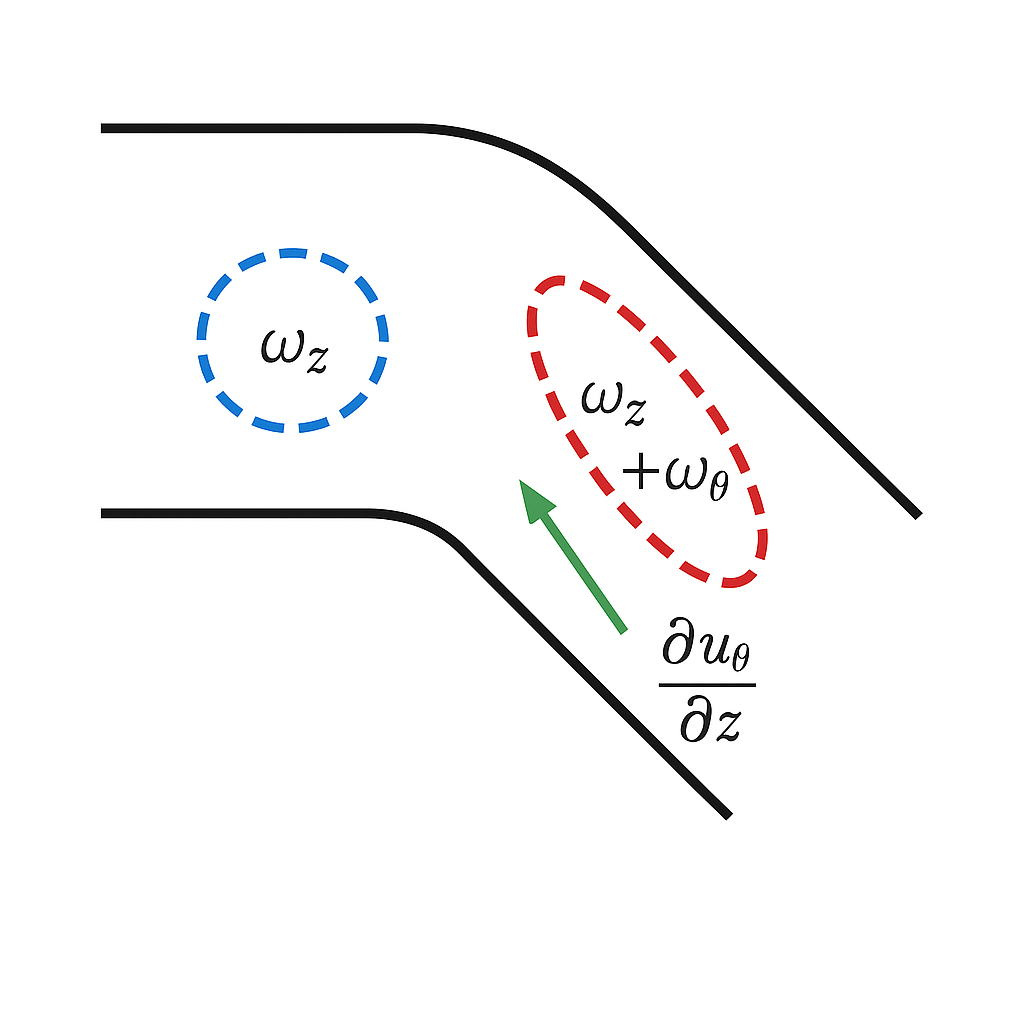
\includegraphics[width=0.6\textwidth]{vorticidad 45.png}
\end{figure}

\subsection{Hipótesis}
\begin{itemize}
    \item Flujo incompresible (densidad constante, $\rho = ct$) y laminar ($Re < 2300$)
    \item Fluido newtoniano (deformación por esfueraos cortantes proporcional al gradiente de velocdiades ($\tau = \mu \frac{du}{dy}$) \& viscosidad $\mu$ constante) 
    \item Simetría axial en el ducto
    \item Geometría curvada suave y constante
    \item Efectos gravitacionales despreciables
\end{itemize}

\subsection{Configuración}
La geometría del conducto provoca un gradiente de velocdidades de manera que en la pared exterior la distancia que debe recorrer 
el fluido aumenta, mientras que en la pared interior disminuye. Esto provoca que las velocidades aumenten en la pared externa y disminuya 
en la interna para conservar el caudal.\\

\textbf{Término dominante:}
\[
(\vec{\omega} \cdot \nabla)\vec{u} \quad \text{(tilting y stretching)}
\]

\textbf{Justificación:}
\begin{itemize}
    \item El flujo sigue una trayectoria curva, generando una componente transversal de velocidad $u_\theta$ que varía en la dirección axial ($z$).
    \item Esto da lugar a un término de deformación de vorticidad:
    \[
    (\vec{\omega} \cdot \nabla)\vec{u} \approx \omega_z \frac{\partial u_\theta}{\partial z}
    \]
    \item El resultado es la transformación de vorticidad axial en vorticidad transversal, formando estructuras secundarias como las células de Dean.
    \item Aunque existe difusión viscosa, esta es secundaria frente a la generación activa de nueva vorticidad.
\end{itemize}

\textbf{Conclusión:} En geometrías curvadas, la curvatura induce mecanismos de inclinación y estiramiento que dominan la evolución de la vorticidad.

\vspace{1em}

El flujo curvado genera un gradiente de velocidad angular $\frac{\partial u_\theta}{\partial z}$, lo cual produce una vorticidad secundaria.

\subsection{Desarrollo Matemático}
En coordenadas cilíndricas $(r,\theta,z)$ y asumiendo que $\omega_z$ es la componente inicial dominante dado que :

\begin{equation}
    (\vec{\omega} \cdot \nabla)\vec{u} = \omega_z \left(
        \frac{\partial u_r}{\partial z} \hat{e}_r +
        \frac{\partial u_\theta}{\partial z} \hat{e}_\theta +
        \frac{\partial u_z}{\partial z} \hat{e}_z
    \right)
\end{equation}

Por simplificación física y geométrica:
\[
\frac{\partial u_r}{\partial z} \ll \frac{\partial u_\theta}{\partial z}, \quad \frac{\partial u_z}{\partial z} \approx 0
\]

Por tanto, el término dominante:
\begin{equation}
    (\vec{\omega} \cdot \nabla)\vec{u} \approx \omega_z \frac{\partial u_\theta}{\partial z} \hat{e}_\theta
\end{equation}

\subsection{Evolución Temporal de la Vorticidad}
Aproximando el gradiente como:
\begin{equation}
    \frac{\partial u_\theta}{\partial z} \approx \frac{\Omega (r_o - r_i)}{L_c} = \frac{\Omega \Delta r}{L_c}
\end{equation}

Entonces:
\begin{equation}
    \frac{D\omega_\theta}{Dt} \approx \omega_z \frac{\Omega \Delta r}{L_c} - \nu \left(\frac{\omega_\theta}{r^2}\right)
\end{equation}


\begin{itemize}
    \item \textbf{Estado inicial:} Vorticidad principalmente axial, $\vec{\omega} \approx \omega_z \hat{e}_z$. Se forma un anillo de vorticidad simétrico en un plano transversal al flujo.
    
    \item \textbf{Al ingresar a la curva:} Aparece un gradiente de velocidad azimutal:
    \[
    \frac{\partial u_\theta}{\partial z} \neq 0
    \]
    debido a la geometría curvada del ducto.
    
    \item \textbf{Término dominante:} Estiramiento y tilting de la vorticidad axial:
    \[
    (\vec{\omega} \cdot \nabla)\vec{u} \approx \omega_z \frac{\partial u_\theta}{\partial z} \hat{e}_\theta
    \]
    lo que genera una nueva componente de vorticidad en la dirección azimutal ($\omega_\theta$).
    
    \item \textbf{Resultado:} El anillo de vorticidad se deforma, adquiere forma elíptica y se inclina, evolucionando hacia una estructura helicoidal. Aparece vorticidad secundaria inducida por la curvatura.
\end{itemize}


\textbf{Conclusión:} la curvatura genera una componente $\omega_\theta$ debido al estiramiento de vorticidad axial. Esto genera estructuras de vorticidad secundaria como pares de vórtices.


\section{Caso 2: Ducto que se Ensancha}

\subsection{Hipótesis}

\begin{center}
    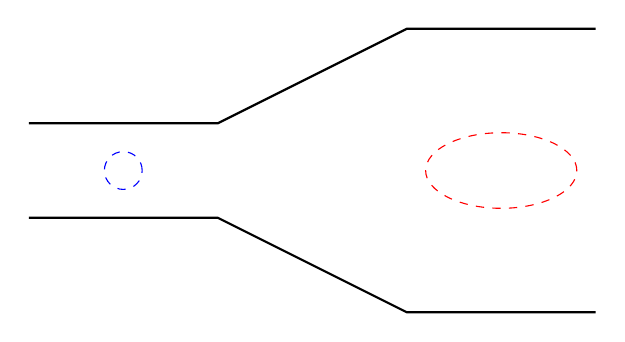
\begin{tikzpicture}[scale=1.2]
        % Ducto que se ensancha
        \draw[thick] (0,-2) -- (2,-2) -- (4,-3) -- (6,-3);
        \draw[thick] (0,-1) -- (2,-1) -- (4,0) -- (6,0);
        
        % Vórtices
        \draw[dashed, blue] (1,-1.5) circle (0.2);
        \draw[dashed, red] (5,-1.5) ellipse (0.8 and 0.4);
    \end{tikzpicture}
    \end{center}

\begin{itemize}
    \item Expansión gradual del área transversal $A(z)$
    \item Conservación de caudal: $Q = A(z)u_z(z)$
    \item Vorticidad inicial puramente axial: $\vec{\omega}(0) = \omega_0 \hat{e}_z$
    \item Flujo incompresible y laminar
\end{itemize}

\textbf{Término dominante:}
\[
\nu \nabla^2 \vec{\omega} \quad \text{(difusión viscosa)}
\]

\textbf{Justificación:}
\begin{itemize}
    \item La expansión del ducto es suave, sin curvatura significativa ni grandes variaciones transversales de velocidad.
    \item La vorticidad inicial es puramente axial y no se generan nuevas componentes por estiramiento o inclinación.
    \item Al aumentar el área de la sección, la velocidad axial disminuye y la vorticidad tiende a disiparse.
    \item Por lo tanto, el comportamiento está gobernado por la difusión de vorticidad:
    \[
    \frac{\partial \omega_z}{\partial t} \approx \nu \nabla^2 \omega_z
    \]
\end{itemize}

\textbf{Conclusión:} En ductos expansivos, la difusión viscosa controla la evolución de la vorticidad al no existir mecanismos activos que la regeneren.


\subsection{Evolución de la Vorticidad}

La ecuación simplificada en coordenadas cilíndricas es:

\begin{equation}
    \frac{\partial \omega_z}{\partial t} + u_z \frac{\partial \omega_z}{\partial z} = \frac{\nu}{r} \frac{\partial}{\partial r} \left( r \frac{\partial \omega_z}{\partial r} \right)
\end{equation}

*nota: $\nabla^2 = \frac{1}{r} \frac{\partial}{\partial r} \left( r \frac{\partial}{\partial r} \right) + \frac{1}{r^2} \frac{\partial^2}{\partial \theta^2}$\\


Este tipo de ecuación admite soluciones autosimilares del tipo:

\begin{equation}
    \omega_z(r,t) = \frac{\Gamma_0}{4\pi \nu t} \exp\left(-\frac{r^2}{4\nu t}\right)
\end{equation}

Donde $\Gamma_0$ es la circulación total y el radio característico evoluciona como:

\begin{equation}
    R(t) = \sqrt{R_0^2 + 4\nu t}
\end{equation}

\subsection{Conservación de Circulación}
\begin{equation}
    \Gamma = \int_0^{R(z)} \omega_z \cdot 2\pi r \, dr = \Gamma_0 = \text{cte}
\end{equation}


\begin{itemize}
    \item \textbf{Estado inicial:} Vorticidad puramente axial, concentrada cerca del eje:
    \[
    \omega_z(r,t=0) = \frac{\Gamma_0}{4\pi \nu t} \exp\left(-\frac{r^2}{4\nu t}\right)
    \]
    
    \item \textbf{Efecto de la expansión:} El área transversal aumenta con $z$, lo que reduce la velocidad axial por conservación del caudal. La vorticidad no se inclina ni estira, sino que se difunde:
    \[
    \frac{\partial \omega_z}{\partial t} \approx \frac{\nu}{r} \frac{\partial}{\partial r} \left( r \frac{\partial \omega_z}{\partial r} \right)
    \]
    
    \item \textbf{Resultado:} El anillo de vorticidad se expande radialmente, disminuye su magnitud pero conserva la circulación:
    \[
    \Gamma = \int_0^{R(z)} \omega_z \cdot 2\pi r \, dr = \Gamma_0
    \]
\end{itemize}

\textbf{Conclusión:} la expansión del ducto causa difusión de la vorticidad axial, ensanchando su perfil radial y reduciendo su magnitud máxima.

\vspace{0.5cm}
\subsection*{Comparación General}

\begin{table}[h]
\centering
\begin{tabular}{|l|c|c|}
\hline
\textbf{Característica} & \textbf{Ducto Curvado} & \textbf{Ducto en Expansión} \\ \hline
Deformación del anillo & Estiramiento + inclinación & Expansión radial \\ \hline
Nuevas componentes de vorticidad & Sí ($\omega_\theta \neq 0$) & No \\ \hline
Mecanismo dominante & Tilting / Stretching & Difusión viscosa \\ \hline
Magnitud de vorticidad & Puede incrementarse localmente & Disminuye globalmente \\ \hline
Circulación total & Conservada & Conservada \\ \hline
\end{tabular}
\caption{Comparación del comportamiento del anillo de vorticidad}
\end{table}



\end{document}
